%----------------------------------------------------------------------------
\section{Behaviour Models}\label{sec:behaviour_models}
%----------------------------------------------------------------------------

\subsection{Finite State Machine}

Finite state machines (FSMs) are widely used formalisms to model computation. They can be in exactly one of a finite number of \emph{states} at any given time. FSM can change from one state to another in response to some \emph{inputs} (usually called signals); which change is called a \emph{transition} (see \autoref{fig:fsm} for an example finite state machine).

\begin{figure}[!ht]
	\centering
	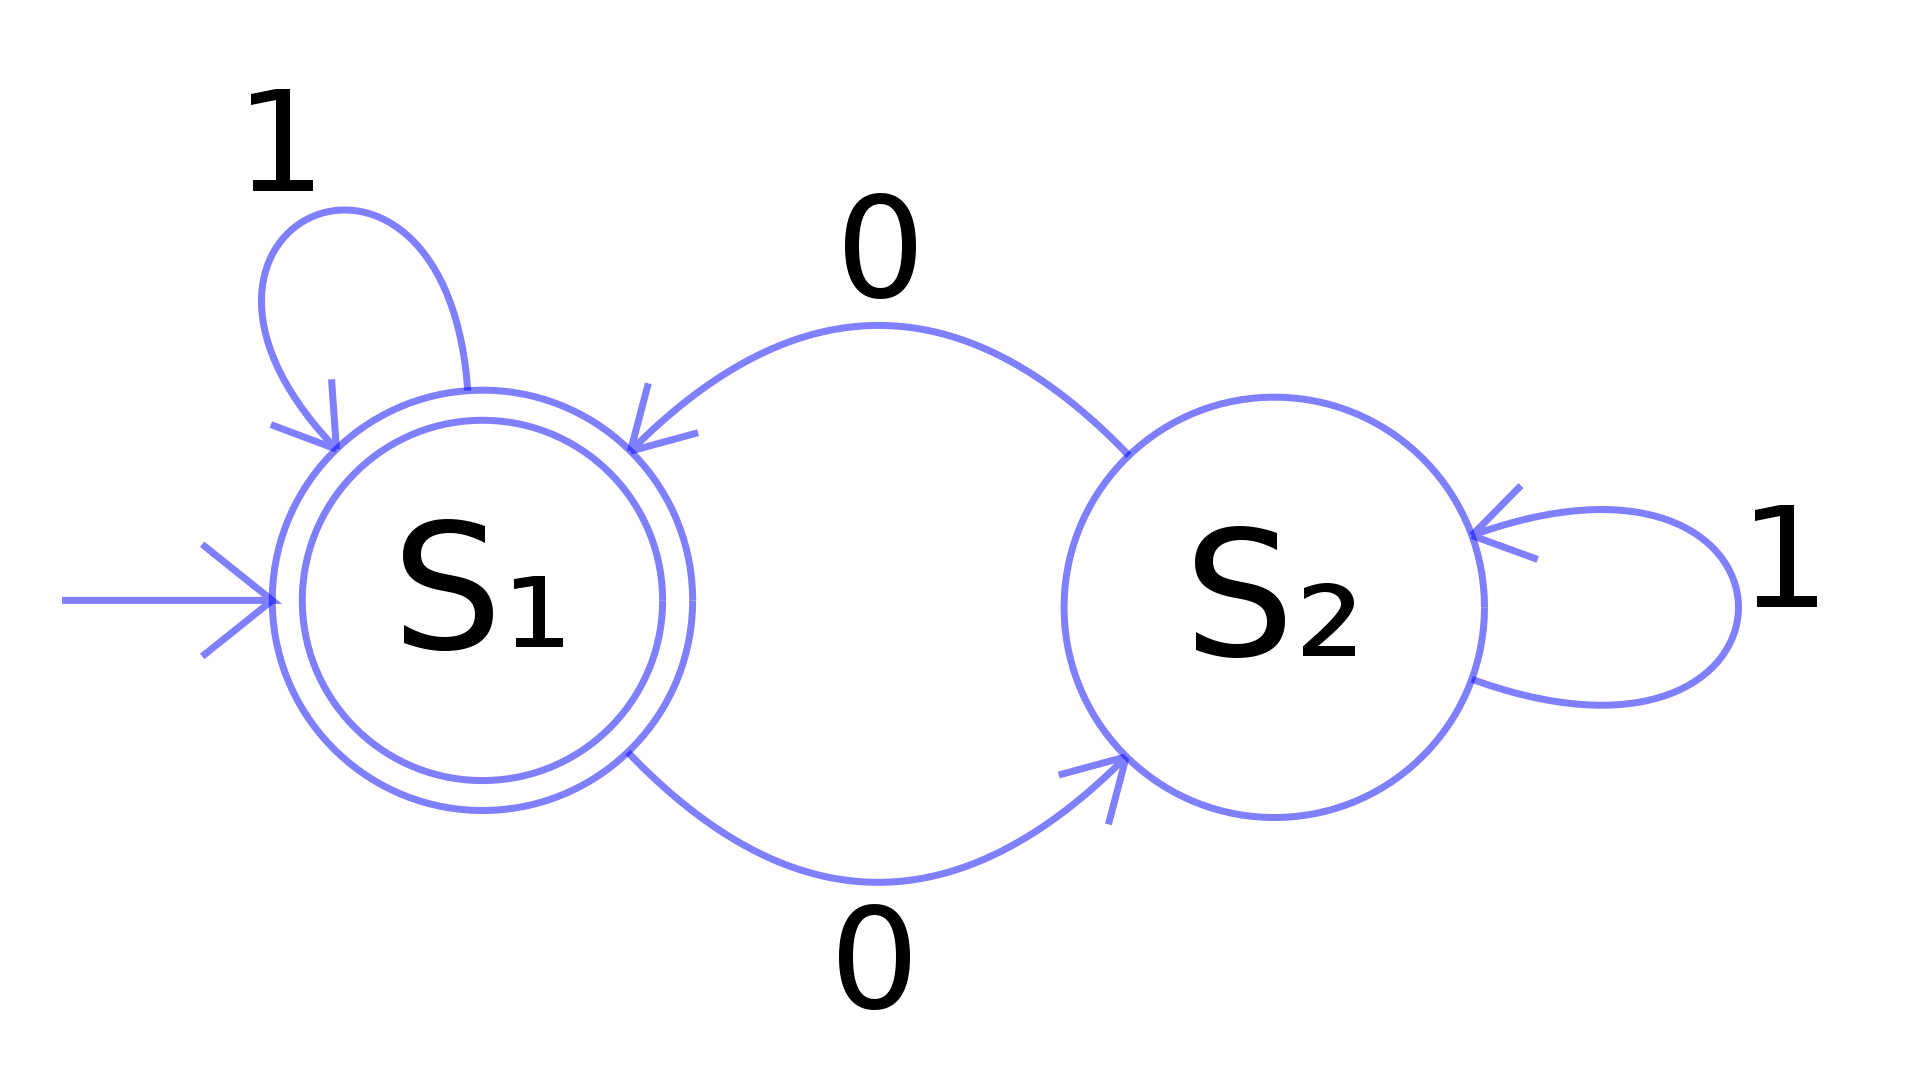
\includegraphics[width=67mm, keepaspectratio]{figures/fsm.png}\hspace{1cm}
	\caption{An example deterministic finite state machine, which checks a given binary numbers \emph{evenness}.}
	\label{fig:fsm}
\end{figure}

The formal definition of \emph{deterministic} finite state machines is as follows.

\begin{definition}[Deterministic finite state machine]
	
	A DFSM is a tuple \( SM = (\Sigma, S, s_0, \delta, F) \)
	
	\begin{itemize}
		\item \(\Sigma\) is the set input \emph{alphabet} (a finite non-empty set of symbols);
		\item \(S\) is a finite non-empty set of states;
		\item \(s_0 \in S\) is an initial state;
		\item \(\delta : S \times \Sigma \rightarrow S \) is the state-transition function;
		\item \(F \subseteq S\) is the set of final states
	\end{itemize}
\end{definition}

The current state of a DFSM is \(s \in S\). A transition from state to state is performed, given the last input letter \(l\), if and only if \( s' = \delta(s, l) \in S \). In which case the current state will become \(s'\) (this work assumes, that if the given \(\delta(s, l)\) is not defined, then the state machine remains in it's current state).
